\documentclass[]{article}
\usepackage{lmodern}
\usepackage{amssymb,amsmath}
\usepackage{ifxetex,ifluatex}
\usepackage{fixltx2e} % provides \textsubscript
\ifnum 0\ifxetex 1\fi\ifluatex 1\fi=0 % if pdftex
  \usepackage[T1]{fontenc}
  \usepackage[utf8]{inputenc}
\else % if luatex or xelatex
  \ifxetex
    \usepackage{mathspec}
  \else
    \usepackage{fontspec}
  \fi
  \defaultfontfeatures{Ligatures=TeX,Scale=MatchLowercase}
\fi
% use upquote if available, for straight quotes in verbatim environments
\IfFileExists{upquote.sty}{\usepackage{upquote}}{}
% use microtype if available
\IfFileExists{microtype.sty}{%
\usepackage{microtype}
\UseMicrotypeSet[protrusion]{basicmath} % disable protrusion for tt fonts
}{}
\usepackage[margin=1in]{geometry}
\usepackage{hyperref}
\hypersetup{unicode=true,
            pdftitle={Neural Networks},
            pdfauthor={Jim Reilly},
            pdfborder={0 0 0},
            breaklinks=true}
\urlstyle{same}  % don't use monospace font for urls
\usepackage{color}
\usepackage{fancyvrb}
\newcommand{\VerbBar}{|}
\newcommand{\VERB}{\Verb[commandchars=\\\{\}]}
\DefineVerbatimEnvironment{Highlighting}{Verbatim}{commandchars=\\\{\}}
% Add ',fontsize=\small' for more characters per line
\usepackage{framed}
\definecolor{shadecolor}{RGB}{248,248,248}
\newenvironment{Shaded}{\begin{snugshade}}{\end{snugshade}}
\newcommand{\KeywordTok}[1]{\textcolor[rgb]{0.13,0.29,0.53}{\textbf{#1}}}
\newcommand{\DataTypeTok}[1]{\textcolor[rgb]{0.13,0.29,0.53}{#1}}
\newcommand{\DecValTok}[1]{\textcolor[rgb]{0.00,0.00,0.81}{#1}}
\newcommand{\BaseNTok}[1]{\textcolor[rgb]{0.00,0.00,0.81}{#1}}
\newcommand{\FloatTok}[1]{\textcolor[rgb]{0.00,0.00,0.81}{#1}}
\newcommand{\ConstantTok}[1]{\textcolor[rgb]{0.00,0.00,0.00}{#1}}
\newcommand{\CharTok}[1]{\textcolor[rgb]{0.31,0.60,0.02}{#1}}
\newcommand{\SpecialCharTok}[1]{\textcolor[rgb]{0.00,0.00,0.00}{#1}}
\newcommand{\StringTok}[1]{\textcolor[rgb]{0.31,0.60,0.02}{#1}}
\newcommand{\VerbatimStringTok}[1]{\textcolor[rgb]{0.31,0.60,0.02}{#1}}
\newcommand{\SpecialStringTok}[1]{\textcolor[rgb]{0.31,0.60,0.02}{#1}}
\newcommand{\ImportTok}[1]{#1}
\newcommand{\CommentTok}[1]{\textcolor[rgb]{0.56,0.35,0.01}{\textit{#1}}}
\newcommand{\DocumentationTok}[1]{\textcolor[rgb]{0.56,0.35,0.01}{\textbf{\textit{#1}}}}
\newcommand{\AnnotationTok}[1]{\textcolor[rgb]{0.56,0.35,0.01}{\textbf{\textit{#1}}}}
\newcommand{\CommentVarTok}[1]{\textcolor[rgb]{0.56,0.35,0.01}{\textbf{\textit{#1}}}}
\newcommand{\OtherTok}[1]{\textcolor[rgb]{0.56,0.35,0.01}{#1}}
\newcommand{\FunctionTok}[1]{\textcolor[rgb]{0.00,0.00,0.00}{#1}}
\newcommand{\VariableTok}[1]{\textcolor[rgb]{0.00,0.00,0.00}{#1}}
\newcommand{\ControlFlowTok}[1]{\textcolor[rgb]{0.13,0.29,0.53}{\textbf{#1}}}
\newcommand{\OperatorTok}[1]{\textcolor[rgb]{0.81,0.36,0.00}{\textbf{#1}}}
\newcommand{\BuiltInTok}[1]{#1}
\newcommand{\ExtensionTok}[1]{#1}
\newcommand{\PreprocessorTok}[1]{\textcolor[rgb]{0.56,0.35,0.01}{\textit{#1}}}
\newcommand{\AttributeTok}[1]{\textcolor[rgb]{0.77,0.63,0.00}{#1}}
\newcommand{\RegionMarkerTok}[1]{#1}
\newcommand{\InformationTok}[1]{\textcolor[rgb]{0.56,0.35,0.01}{\textbf{\textit{#1}}}}
\newcommand{\WarningTok}[1]{\textcolor[rgb]{0.56,0.35,0.01}{\textbf{\textit{#1}}}}
\newcommand{\AlertTok}[1]{\textcolor[rgb]{0.94,0.16,0.16}{#1}}
\newcommand{\ErrorTok}[1]{\textcolor[rgb]{0.64,0.00,0.00}{\textbf{#1}}}
\newcommand{\NormalTok}[1]{#1}
\usepackage{graphicx,grffile}
\makeatletter
\def\maxwidth{\ifdim\Gin@nat@width>\linewidth\linewidth\else\Gin@nat@width\fi}
\def\maxheight{\ifdim\Gin@nat@height>\textheight\textheight\else\Gin@nat@height\fi}
\makeatother
% Scale images if necessary, so that they will not overflow the page
% margins by default, and it is still possible to overwrite the defaults
% using explicit options in \includegraphics[width, height, ...]{}
\setkeys{Gin}{width=\maxwidth,height=\maxheight,keepaspectratio}
\IfFileExists{parskip.sty}{%
\usepackage{parskip}
}{% else
\setlength{\parindent}{0pt}
\setlength{\parskip}{6pt plus 2pt minus 1pt}
}
\setlength{\emergencystretch}{3em}  % prevent overfull lines
\providecommand{\tightlist}{%
  \setlength{\itemsep}{0pt}\setlength{\parskip}{0pt}}
\setcounter{secnumdepth}{0}
% Redefines (sub)paragraphs to behave more like sections
\ifx\paragraph\undefined\else
\let\oldparagraph\paragraph
\renewcommand{\paragraph}[1]{\oldparagraph{#1}\mbox{}}
\fi
\ifx\subparagraph\undefined\else
\let\oldsubparagraph\subparagraph
\renewcommand{\subparagraph}[1]{\oldsubparagraph{#1}\mbox{}}
\fi

%%% Use protect on footnotes to avoid problems with footnotes in titles
\let\rmarkdownfootnote\footnote%
\def\footnote{\protect\rmarkdownfootnote}

%%% Change title format to be more compact
\usepackage{titling}

% Create subtitle command for use in maketitle
\newcommand{\subtitle}[1]{
  \posttitle{
    \begin{center}\large#1\end{center}
    }
}

\setlength{\droptitle}{-2em}

  \title{Neural Networks}
    \pretitle{\vspace{\droptitle}\centering\huge}
  \posttitle{\par}
    \author{Jim Reilly}
    \preauthor{\centering\large\emph}
  \postauthor{\par}
      \predate{\centering\large\emph}
  \postdate{\par}
    \date{April 8, 2019}


\begin{document}
\maketitle

\begin{Shaded}
\begin{Highlighting}[]
\KeywordTok{library}\NormalTok{(neuralnet)}
\KeywordTok{library}\NormalTok{(fastDummies)}
\KeywordTok{library}\NormalTok{(caret)}
\KeywordTok{library}\NormalTok{(dplyr)}
\KeywordTok{library}\NormalTok{(e1071)}
\end{Highlighting}
\end{Shaded}

\subsubsection{11.1 Credit Card Use}\label{credit-card-use}

\begin{figure}
\centering
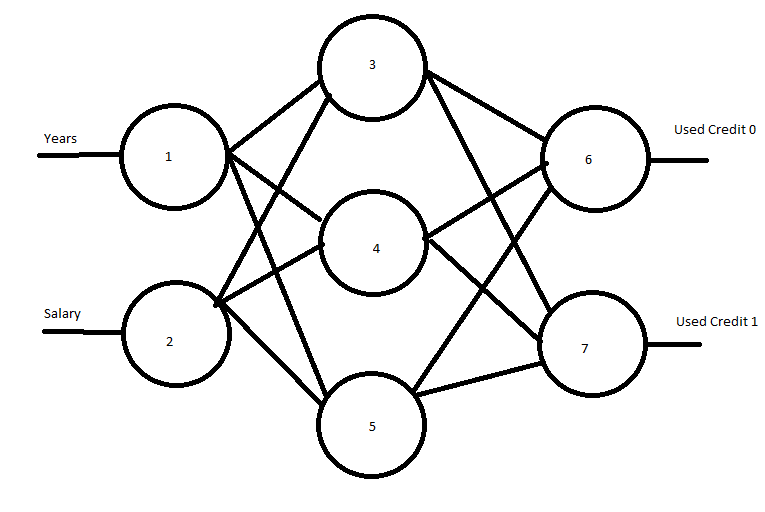
\includegraphics{figures/awful-ann-drawing.png}
\caption{Hand-drawn ANN Model}
\end{figure}

Using this crap drawing of what I will be doing, I will walkthrough the
ANN calculation for 1 set of inputs with random low seeds.

\begin{Shaded}
\begin{Highlighting}[]
\CommentTok{#later 0 (input layer)}
\NormalTok{year <-}\StringTok{ }\DecValTok{4}
\NormalTok{salary <-}\StringTok{ }\DecValTok{43}

\CommentTok{#initial weights and betas}
\NormalTok{w <-}\StringTok{ }\KeywordTok{runif}\NormalTok{(}\DecValTok{12}\NormalTok{, }\OperatorTok{-}\FloatTok{0.05}\NormalTok{,}\FloatTok{0.05}\NormalTok{)}
\NormalTok{b <-}\StringTok{ }\KeywordTok{runif}\NormalTok{(}\DecValTok{5}\NormalTok{, }\OperatorTok{-}\FloatTok{0.3}\NormalTok{,}\FloatTok{0.3}\NormalTok{)}

\CommentTok{#layer 1}
\CommentTok{#node 3 = (4 * w1) + (43 * w2) + beta1}
\CommentTok{#node 4 = (4 * w3) + (43 * w4) + beta2}
\CommentTok{#node 5 = (4 * w5) + (43 * w6) + beta3}

\NormalTok{n3 <-}\StringTok{ }\KeywordTok{sigmoid}\NormalTok{((year }\OperatorTok{*}\StringTok{ }\NormalTok{w[}\DecValTok{1}\NormalTok{]) }\OperatorTok{+}\StringTok{ }\NormalTok{(salary }\OperatorTok{*}\StringTok{ }\NormalTok{w[}\DecValTok{2}\NormalTok{]) }\OperatorTok{+}\StringTok{ }\NormalTok{b[}\DecValTok{1}\NormalTok{])}
\NormalTok{n4 <-}\StringTok{ }\KeywordTok{sigmoid}\NormalTok{((year }\OperatorTok{*}\StringTok{ }\NormalTok{w[}\DecValTok{3}\NormalTok{]) }\OperatorTok{+}\StringTok{ }\NormalTok{(salary }\OperatorTok{*}\StringTok{ }\NormalTok{w[}\DecValTok{4}\NormalTok{]) }\OperatorTok{+}\StringTok{ }\NormalTok{b[}\DecValTok{2}\NormalTok{])}
\NormalTok{n5 <-}\StringTok{ }\KeywordTok{sigmoid}\NormalTok{((year }\OperatorTok{*}\StringTok{ }\NormalTok{w[}\DecValTok{5}\NormalTok{]) }\OperatorTok{+}\StringTok{ }\NormalTok{(salary }\OperatorTok{*}\StringTok{ }\NormalTok{w[}\DecValTok{6}\NormalTok{]) }\OperatorTok{+}\StringTok{ }\NormalTok{b[}\DecValTok{3}\NormalTok{])}

\CommentTok{#layer 2 (output layer)}
\CommentTok{#node 6 = (node3 * w7) + (node4 * w8) + (node5 * w9) + beta4}
\CommentTok{#node 7 = (node3 * w10) + (node4 * w11) + (node5 * w12) + beta5}

\NormalTok{usedCredit.}\DecValTok{0}\NormalTok{ <-}\StringTok{ }\KeywordTok{sigmoid}\NormalTok{((n3 }\OperatorTok{*}\StringTok{ }\NormalTok{w[}\DecValTok{7}\NormalTok{]) }\OperatorTok{+}\StringTok{ }\NormalTok{(n4 }\OperatorTok{*}\StringTok{ }\NormalTok{w[}\DecValTok{8}\NormalTok{]) }\OperatorTok{+}\StringTok{ }\NormalTok{(n5 }\OperatorTok{*}\StringTok{ }\NormalTok{w[}\DecValTok{9}\NormalTok{]) }\OperatorTok{+}\StringTok{ }\NormalTok{b[}\DecValTok{4}\NormalTok{])}
\NormalTok{usedCredit.}\DecValTok{1}\NormalTok{ <-}\StringTok{ }\KeywordTok{sigmoid}\NormalTok{((n3 }\OperatorTok{*}\StringTok{ }\NormalTok{w[}\DecValTok{10}\NormalTok{]) }\OperatorTok{+}\StringTok{ }\NormalTok{(n4 }\OperatorTok{*}\StringTok{ }\NormalTok{w[}\DecValTok{11}\NormalTok{]) }\OperatorTok{+}\StringTok{ }\NormalTok{(n5 }\OperatorTok{*}\StringTok{ }\NormalTok{w[}\DecValTok{12}\NormalTok{]) }\OperatorTok{+}\StringTok{ }\NormalTok{b[}\DecValTok{5}\NormalTok{])}

\CommentTok{#adjust the values to add to 1.0}

\NormalTok{usedCredit.}\DecValTok{0}\NormalTok{ <-}\StringTok{ }\NormalTok{usedCredit.}\DecValTok{0} \OperatorTok{/}\StringTok{ }\NormalTok{(usedCredit.}\DecValTok{0} \OperatorTok{+}\StringTok{ }\NormalTok{usedCredit.}\DecValTok{1}\NormalTok{)}
\NormalTok{usedCredit.}\DecValTok{1}\NormalTok{ <-}\StringTok{ }\DecValTok{1} \OperatorTok{-}\StringTok{ }\NormalTok{usedCredit.}\DecValTok{0}
\end{Highlighting}
\end{Shaded}

The calculated values with random weights and biases are 0.5493069 and
0.4506931. We can compare this to the known value of the input 0 and
adjust the weights accordingly to increase the 0 rating and decrease the
1 rating

\subsubsection{11.2 Neural Net Evolution}\label{neural-net-evolution}

As stated, ANNs start with typically random starting seed which account
for the variation in training result each time. What allows all ANNs to
converge in accuracy regardless of seed is backpropogation. Back
propogation is the process of adjusting the weights into a layer of
nodes after the calculation is complete in order to increase the desired
class and decrease the incorrect classes propensity scores for a given
input. This weight adjustment can be taken at each layer all the way
back to the original set of inputs and for all different inputs. Each
round of backpropogation increases the performance of the model and
reduces the model's error until the error cannot be improved and the
model has efficiently ``learned'' the training data. When considering
backpropogation for a set of input data the adjustments made are the
average of all individual calculated adjustments, then another round of
training can continue. This is called case updating (updating for 1
input) vs.~batch updating (for a set of inputs)

Back propogation can stop after a certain minimum predetermined
threshold of change in the weights is not met or a target classification
error is reached, or after a predetermined number of rounds.

\subsubsection{11.3 Toyota Corolla}\label{toyota-corolla}

In the below excercise I train a series of ANNs on a set of data
relating to the sale of Toyota Corollas. I use the exact same parameters
in each model and modify only the number of hidden layers and the
dimensions of those layers.

First I load the dataset and normalize all columns before splitting the
data into test and validation sets.

Next I train 4 ANNs, All discussion is beneath the last ANN validations.

The notation below indicates how many nodes there are from the input
layer (17) to the output layer (1) 1) 17-2-1 2) 17-5-1 3) 17-5-5-1 4)
17-13-13-13-13-13-5-1

\begin{Shaded}
\begin{Highlighting}[]
\NormalTok{toyota <-}\StringTok{ }\KeywordTok{read.csv}\NormalTok{(}\StringTok{"data/ToyotaCorolla.csv"}\NormalTok{)}

\NormalTok{toyota <-}\StringTok{ }\NormalTok{fastDummies}\OperatorTok{::}\KeywordTok{dummy_cols}\NormalTok{(toyota, }\DataTypeTok{select_columns =} \StringTok{"Fuel_Type"}\NormalTok{)}
\NormalTok{toyota <-}\StringTok{ }\NormalTok{toyota }\OperatorTok\StringTok{ }\KeywordTok{select}\NormalTok{(Price,Age_08_}\DecValTok{04}\NormalTok{,KM,Fuel_Type_Diesel,Fuel_Type_Petrol,Fuel_Type_CNG,HP,Automatic,Doors,Quarterly_Tax,Mfr_Guarantee,Guarantee_Period,Airco,Automatic_airco,CD_Player,Powered_Windows,Sport_Model,Tow_Bar)}

\NormalTok{maxs <-}\StringTok{ }\KeywordTok{apply}\NormalTok{(toyota, }\DecValTok{2}\NormalTok{, max) }
\NormalTok{mins <-}\StringTok{ }\KeywordTok{apply}\NormalTok{(toyota, }\DecValTok{2}\NormalTok{, min)}
\NormalTok{toyota.range <-}\StringTok{ }\KeywordTok{as.data.frame}\NormalTok{(}\KeywordTok{scale}\NormalTok{(toyota, }\DataTypeTok{center =}\NormalTok{ mins, }\DataTypeTok{scale =}\NormalTok{ maxs }\OperatorTok{-}\StringTok{ }\NormalTok{mins))}

\NormalTok{trainIndex <-}\StringTok{ }\KeywordTok{createDataPartition}\NormalTok{(toyota}\OperatorTok{$}\NormalTok{Price, }\DataTypeTok{p =} \FloatTok{0.8}\NormalTok{, }\DataTypeTok{list =} \OtherTok{FALSE}\NormalTok{)}
\NormalTok{toyota.range.train <-}\StringTok{ }\NormalTok{toyota.range[trainIndex, ]}
\NormalTok{toyota.range.valid <-}\StringTok{ }\NormalTok{toyota.range[}\OperatorTok{-}\NormalTok{trainIndex, ]}
\end{Highlighting}
\end{Shaded}

\begin{Shaded}
\begin{Highlighting}[]
\NormalTok{trainstart <-}\StringTok{ }\KeywordTok{Sys.time}\NormalTok{();}
\NormalTok{toyota.nn <-}\StringTok{ }\KeywordTok{neuralnet}\NormalTok{(}\DataTypeTok{formula =}\NormalTok{ Price }\OperatorTok{~}\StringTok{ }\NormalTok{Age_08_}\DecValTok{04} \OperatorTok{+}\StringTok{ }\NormalTok{KM }\OperatorTok{+}\StringTok{ }\NormalTok{Fuel_Type_Diesel }\OperatorTok{+}\StringTok{ }\NormalTok{Fuel_Type_Petrol }\OperatorTok{+}\StringTok{ }\NormalTok{Fuel_Type_CNG }\OperatorTok{+}\StringTok{ }\NormalTok{HP }\OperatorTok{+}\StringTok{ }\NormalTok{Automatic }\OperatorTok{+}\StringTok{ }\NormalTok{Doors }\OperatorTok{+}\StringTok{ }\NormalTok{Quarterly_Tax }\OperatorTok{+}\StringTok{ }\NormalTok{Mfr_Guarantee }\OperatorTok{+}\StringTok{ }\NormalTok{Guarantee_Period }\OperatorTok{+}\StringTok{ }\NormalTok{Airco }\OperatorTok{+}\StringTok{ }\NormalTok{Automatic_airco }\OperatorTok{+}\StringTok{ }\NormalTok{CD_Player }\OperatorTok{+}\StringTok{ }\NormalTok{Powered_Windows }\OperatorTok{+}\StringTok{ }\NormalTok{Sport_Model }\OperatorTok{+}\StringTok{ }\NormalTok{Tow_Bar, }\DataTypeTok{data =}\NormalTok{ toyota.range.train, }\DataTypeTok{hidden =} \DecValTok{2}\NormalTok{, }\DataTypeTok{linear.output =}\NormalTok{ T)}
\KeywordTok{Sys.time}\NormalTok{() }\OperatorTok{-}\StringTok{ }\NormalTok{trainstart}
\end{Highlighting}
\end{Shaded}

\begin{verbatim}
## Time difference of 5.375863075 secs
\end{verbatim}

\begin{Shaded}
\begin{Highlighting}[]
\CommentTok{#drop the Price column because its the predicted value}
\NormalTok{toyota.training.pred <-}\StringTok{ }\NormalTok{neuralnet}\OperatorTok{::}\KeywordTok{compute}\NormalTok{(toyota.nn, toyota.range.train[,}\DecValTok{2}\OperatorTok{:}\DecValTok{18}\NormalTok{])}

\NormalTok{toyota.training.predictions <-}\StringTok{ }\NormalTok{toyota.training.pred}\OperatorTok{$}\NormalTok{net.result}\OperatorTok{*}\NormalTok{(}\KeywordTok{max}\NormalTok{(toyota}\OperatorTok{$}\NormalTok{Price)}\OperatorTok{-}\KeywordTok{min}\NormalTok{(toyota}\OperatorTok{$}\NormalTok{Price))}\OperatorTok{+}\KeywordTok{min}\NormalTok{(toyota}\OperatorTok{$}\NormalTok{Price)}
\NormalTok{toyota.training.actuals <-}\StringTok{ }\NormalTok{toyota[trainIndex,}\DecValTok{1}\NormalTok{]}

\CommentTok{#training set RMSE}
\KeywordTok{RMSE}\NormalTok{(toyota.training.predictions, toyota.training.actuals)}
\end{Highlighting}
\end{Shaded}

\begin{verbatim}
## [1] 1027.776716
\end{verbatim}

\begin{Shaded}
\begin{Highlighting}[]
\NormalTok{toyota.validation.pred <-}\StringTok{ }\NormalTok{neuralnet}\OperatorTok{::}\KeywordTok{compute}\NormalTok{(toyota.nn, toyota.range.valid[,}\DecValTok{2}\OperatorTok{:}\DecValTok{18}\NormalTok{])}

\NormalTok{toyota.validation.predictions <-}\StringTok{ }\NormalTok{toyota.validation.pred}\OperatorTok{$}\NormalTok{net.result}\OperatorTok{*}\NormalTok{(}\KeywordTok{max}\NormalTok{(toyota}\OperatorTok{$}\NormalTok{Price)}\OperatorTok{-}\KeywordTok{min}\NormalTok{(toyota}\OperatorTok{$}\NormalTok{Price))}\OperatorTok{+}\KeywordTok{min}\NormalTok{(toyota}\OperatorTok{$}\NormalTok{Price)}
\NormalTok{toyota.validation.actuals <-}\StringTok{ }\NormalTok{toyota[}\OperatorTok{-}\NormalTok{trainIndex,}\DecValTok{1}\NormalTok{]}

\CommentTok{#validation set RMSE}
\KeywordTok{RMSE}\NormalTok{(toyota.validation.predictions, toyota.validation.actuals)}
\end{Highlighting}
\end{Shaded}

\begin{verbatim}
## [1] 1089.256737
\end{verbatim}

\begin{Shaded}
\begin{Highlighting}[]
\NormalTok{trainstart <-}\StringTok{ }\KeywordTok{Sys.time}\NormalTok{();}
\NormalTok{toyota.nn <-}\StringTok{ }\KeywordTok{neuralnet}\NormalTok{(}\DataTypeTok{formula =}\NormalTok{ Price }\OperatorTok{~}\StringTok{ }\NormalTok{Age_08_}\DecValTok{04} \OperatorTok{+}\StringTok{ }\NormalTok{KM }\OperatorTok{+}\StringTok{ }\NormalTok{Fuel_Type_Diesel }\OperatorTok{+}\StringTok{ }\NormalTok{Fuel_Type_Petrol }\OperatorTok{+}\StringTok{ }\NormalTok{Fuel_Type_CNG }\OperatorTok{+}\StringTok{ }\NormalTok{HP }\OperatorTok{+}\StringTok{ }\NormalTok{Automatic }\OperatorTok{+}\StringTok{ }\NormalTok{Doors }\OperatorTok{+}\StringTok{ }\NormalTok{Quarterly_Tax }\OperatorTok{+}\StringTok{ }\NormalTok{Mfr_Guarantee }\OperatorTok{+}\StringTok{ }\NormalTok{Guarantee_Period }\OperatorTok{+}\StringTok{ }\NormalTok{Airco }\OperatorTok{+}\StringTok{ }\NormalTok{Automatic_airco }\OperatorTok{+}\StringTok{ }\NormalTok{CD_Player }\OperatorTok{+}\StringTok{ }\NormalTok{Powered_Windows }\OperatorTok{+}\StringTok{ }\NormalTok{Sport_Model }\OperatorTok{+}\StringTok{ }\NormalTok{Tow_Bar, }\DataTypeTok{data =}\NormalTok{ toyota.range.train, }\DataTypeTok{hidden =} \DecValTok{5}\NormalTok{, }\DataTypeTok{linear.output =}\NormalTok{ T)}
\KeywordTok{Sys.time}\NormalTok{() }\OperatorTok{-}\StringTok{ }\NormalTok{trainstart}
\end{Highlighting}
\end{Shaded}

\begin{verbatim}
## Time difference of 5.369748116 secs
\end{verbatim}

\begin{Shaded}
\begin{Highlighting}[]
\CommentTok{#drop the Price column because its the predicted value}
\NormalTok{toyota.training.pred <-}\StringTok{ }\NormalTok{neuralnet}\OperatorTok{::}\KeywordTok{compute}\NormalTok{(toyota.nn, toyota.range.train[,}\DecValTok{2}\OperatorTok{:}\DecValTok{18}\NormalTok{])}

\NormalTok{toyota.training.predictions <-}\StringTok{ }\NormalTok{toyota.training.pred}\OperatorTok{$}\NormalTok{net.result}\OperatorTok{*}\NormalTok{(}\KeywordTok{max}\NormalTok{(toyota}\OperatorTok{$}\NormalTok{Price)}\OperatorTok{-}\KeywordTok{min}\NormalTok{(toyota}\OperatorTok{$}\NormalTok{Price))}\OperatorTok{+}\KeywordTok{min}\NormalTok{(toyota}\OperatorTok{$}\NormalTok{Price)}
\NormalTok{toyota.training.actuals <-}\StringTok{ }\NormalTok{toyota[trainIndex,}\DecValTok{1}\NormalTok{]}

\CommentTok{#training set RMSE}
\KeywordTok{RMSE}\NormalTok{(toyota.training.predictions, toyota.training.actuals)}
\end{Highlighting}
\end{Shaded}

\begin{verbatim}
## [1] 929.8578434
\end{verbatim}

\begin{Shaded}
\begin{Highlighting}[]
\NormalTok{toyota.validation.pred <-}\StringTok{ }\NormalTok{neuralnet}\OperatorTok{::}\KeywordTok{compute}\NormalTok{(toyota.nn, toyota.range.valid[,}\DecValTok{2}\OperatorTok{:}\DecValTok{18}\NormalTok{])}

\NormalTok{toyota.validation.predictions <-}\StringTok{ }\NormalTok{toyota.validation.pred}\OperatorTok{$}\NormalTok{net.result}\OperatorTok{*}\NormalTok{(}\KeywordTok{max}\NormalTok{(toyota}\OperatorTok{$}\NormalTok{Price)}\OperatorTok{-}\KeywordTok{min}\NormalTok{(toyota}\OperatorTok{$}\NormalTok{Price))}\OperatorTok{+}\KeywordTok{min}\NormalTok{(toyota}\OperatorTok{$}\NormalTok{Price)}
\NormalTok{toyota.validation.actuals <-}\StringTok{ }\NormalTok{toyota[}\OperatorTok{-}\NormalTok{trainIndex,}\DecValTok{1}\NormalTok{]}

\CommentTok{#validation set RMSE}
\KeywordTok{RMSE}\NormalTok{(toyota.validation.predictions, toyota.validation.actuals)}
\end{Highlighting}
\end{Shaded}

\begin{verbatim}
## [1] 1164.691737
\end{verbatim}

\begin{Shaded}
\begin{Highlighting}[]
\NormalTok{trainstart <-}\StringTok{ }\KeywordTok{Sys.time}\NormalTok{();}
\NormalTok{toyota.nn <-}\StringTok{ }\KeywordTok{neuralnet}\NormalTok{(}\DataTypeTok{formula =}\NormalTok{ Price }\OperatorTok{~}\StringTok{ }\NormalTok{Age_08_}\DecValTok{04} \OperatorTok{+}\StringTok{ }\NormalTok{KM }\OperatorTok{+}\StringTok{ }\NormalTok{Fuel_Type_Diesel }\OperatorTok{+}\StringTok{ }\NormalTok{Fuel_Type_Petrol }\OperatorTok{+}\StringTok{ }\NormalTok{Fuel_Type_CNG }\OperatorTok{+}\StringTok{ }\NormalTok{HP }\OperatorTok{+}\StringTok{ }\NormalTok{Automatic }\OperatorTok{+}\StringTok{ }\NormalTok{Doors }\OperatorTok{+}\StringTok{ }\NormalTok{Quarterly_Tax }\OperatorTok{+}\StringTok{ }\NormalTok{Mfr_Guarantee }\OperatorTok{+}\StringTok{ }\NormalTok{Guarantee_Period }\OperatorTok{+}\StringTok{ }\NormalTok{Airco }\OperatorTok{+}\StringTok{ }\NormalTok{Automatic_airco }\OperatorTok{+}\StringTok{ }\NormalTok{CD_Player }\OperatorTok{+}\StringTok{ }\NormalTok{Powered_Windows }\OperatorTok{+}\StringTok{ }\NormalTok{Sport_Model }\OperatorTok{+}\StringTok{ }\NormalTok{Tow_Bar, }\DataTypeTok{data =}\NormalTok{ toyota.range.train, }\DataTypeTok{hidden =} \KeywordTok{c}\NormalTok{(}\DecValTok{5}\NormalTok{,}\DecValTok{5}\NormalTok{), }\DataTypeTok{linear.output =}\NormalTok{ T)}
\KeywordTok{Sys.time}\NormalTok{() }\OperatorTok{-}\StringTok{ }\NormalTok{trainstart}
\end{Highlighting}
\end{Shaded}

\begin{verbatim}
## Time difference of 1.099729061 secs
\end{verbatim}

\begin{Shaded}
\begin{Highlighting}[]
\CommentTok{#drop the Price column because its the predicted value}
\NormalTok{toyota.training.pred <-}\StringTok{ }\NormalTok{neuralnet}\OperatorTok{::}\KeywordTok{compute}\NormalTok{(toyota.nn, toyota.range.train[,}\DecValTok{2}\OperatorTok{:}\DecValTok{18}\NormalTok{])}

\NormalTok{toyota.training.predictions <-}\StringTok{ }\NormalTok{toyota.training.pred}\OperatorTok{$}\NormalTok{net.result}\OperatorTok{*}\NormalTok{(}\KeywordTok{max}\NormalTok{(toyota}\OperatorTok{$}\NormalTok{Price)}\OperatorTok{-}\KeywordTok{min}\NormalTok{(toyota}\OperatorTok{$}\NormalTok{Price))}\OperatorTok{+}\KeywordTok{min}\NormalTok{(toyota}\OperatorTok{$}\NormalTok{Price)}
\NormalTok{toyota.training.actuals <-}\StringTok{ }\NormalTok{toyota[trainIndex,}\DecValTok{1}\NormalTok{]}

\CommentTok{#training set RMSE}
\KeywordTok{RMSE}\NormalTok{(toyota.training.predictions, toyota.training.actuals)}
\end{Highlighting}
\end{Shaded}

\begin{verbatim}
## [1] 994.8246536
\end{verbatim}

\begin{Shaded}
\begin{Highlighting}[]
\NormalTok{toyota.validation.pred <-}\StringTok{ }\NormalTok{neuralnet}\OperatorTok{::}\KeywordTok{compute}\NormalTok{(toyota.nn, toyota.range.valid[,}\DecValTok{2}\OperatorTok{:}\DecValTok{18}\NormalTok{])}

\NormalTok{toyota.validation.predictions <-}\StringTok{ }\NormalTok{toyota.validation.pred}\OperatorTok{$}\NormalTok{net.result}\OperatorTok{*}\NormalTok{(}\KeywordTok{max}\NormalTok{(toyota}\OperatorTok{$}\NormalTok{Price)}\OperatorTok{-}\KeywordTok{min}\NormalTok{(toyota}\OperatorTok{$}\NormalTok{Price))}\OperatorTok{+}\KeywordTok{min}\NormalTok{(toyota}\OperatorTok{$}\NormalTok{Price)}
\NormalTok{toyota.validation.actuals <-}\StringTok{ }\NormalTok{toyota[}\OperatorTok{-}\NormalTok{trainIndex,}\DecValTok{1}\NormalTok{]}

\CommentTok{#validation set RMSE}
\KeywordTok{RMSE}\NormalTok{(toyota.validation.predictions, toyota.validation.actuals)}
\end{Highlighting}
\end{Shaded}

\begin{verbatim}
## [1] 1082.062624
\end{verbatim}

\begin{Shaded}
\begin{Highlighting}[]
\NormalTok{trainstart <-}\StringTok{ }\KeywordTok{Sys.time}\NormalTok{();}
\NormalTok{toyota.nn <-}\StringTok{ }\KeywordTok{neuralnet}\NormalTok{(}\DataTypeTok{formula =}\NormalTok{ Price }\OperatorTok{~}\StringTok{ }\NormalTok{Age_08_}\DecValTok{04} \OperatorTok{+}\StringTok{ }\NormalTok{KM }\OperatorTok{+}\StringTok{ }\NormalTok{Fuel_Type_Diesel }\OperatorTok{+}\StringTok{ }\NormalTok{Fuel_Type_Petrol }\OperatorTok{+}\StringTok{ }\NormalTok{Fuel_Type_CNG }\OperatorTok{+}\StringTok{ }\NormalTok{HP }\OperatorTok{+}\StringTok{ }\NormalTok{Automatic }\OperatorTok{+}\StringTok{ }\NormalTok{Doors }\OperatorTok{+}\StringTok{ }\NormalTok{Quarterly_Tax }\OperatorTok{+}\StringTok{ }\NormalTok{Mfr_Guarantee }\OperatorTok{+}\StringTok{ }\NormalTok{Guarantee_Period }\OperatorTok{+}\StringTok{ }\NormalTok{Airco }\OperatorTok{+}\StringTok{ }\NormalTok{Automatic_airco }\OperatorTok{+}\StringTok{ }\NormalTok{CD_Player }\OperatorTok{+}\StringTok{ }\NormalTok{Powered_Windows }\OperatorTok{+}\StringTok{ }\NormalTok{Sport_Model }\OperatorTok{+}\StringTok{ }\NormalTok{Tow_Bar, }\DataTypeTok{data =}\NormalTok{ toyota.range.train, }\DataTypeTok{hidden =} \KeywordTok{c}\NormalTok{(}\DecValTok{13}\NormalTok{,}\DecValTok{13}\NormalTok{,}\DecValTok{13}\NormalTok{,}\DecValTok{13}\NormalTok{,}\DecValTok{13}\NormalTok{,}\DecValTok{5}\NormalTok{), }\DataTypeTok{linear.output =}\NormalTok{ T)}
\KeywordTok{Sys.time}\NormalTok{() }\OperatorTok{-}\StringTok{ }\NormalTok{trainstart}
\end{Highlighting}
\end{Shaded}

\begin{verbatim}
## Time difference of 4.434206009 secs
\end{verbatim}

\begin{Shaded}
\begin{Highlighting}[]
\CommentTok{#drop the Price column because its the predicted value}
\NormalTok{toyota.training.pred <-}\StringTok{ }\NormalTok{neuralnet}\OperatorTok{::}\KeywordTok{compute}\NormalTok{(toyota.nn, toyota.range.train[,}\DecValTok{2}\OperatorTok{:}\DecValTok{18}\NormalTok{])}

\NormalTok{toyota.training.predictions <-}\StringTok{ }\NormalTok{toyota.training.pred}\OperatorTok{$}\NormalTok{net.result}\OperatorTok{*}\NormalTok{(}\KeywordTok{max}\NormalTok{(toyota}\OperatorTok{$}\NormalTok{Price)}\OperatorTok{-}\KeywordTok{min}\NormalTok{(toyota}\OperatorTok{$}\NormalTok{Price))}\OperatorTok{+}\KeywordTok{min}\NormalTok{(toyota}\OperatorTok{$}\NormalTok{Price)}
\NormalTok{toyota.training.actuals <-}\StringTok{ }\NormalTok{toyota[trainIndex,}\DecValTok{1}\NormalTok{]}

\CommentTok{#training set RMSE}
\KeywordTok{RMSE}\NormalTok{(toyota.training.predictions, toyota.training.actuals)}
\end{Highlighting}
\end{Shaded}

\begin{verbatim}
## [1] 856.5510077
\end{verbatim}

\begin{Shaded}
\begin{Highlighting}[]
\NormalTok{toyota.validation.pred <-}\StringTok{ }\NormalTok{neuralnet}\OperatorTok{::}\KeywordTok{compute}\NormalTok{(toyota.nn, toyota.range.valid[,}\DecValTok{2}\OperatorTok{:}\DecValTok{18}\NormalTok{])}

\NormalTok{toyota.validation.predictions <-}\StringTok{ }\NormalTok{toyota.validation.pred}\OperatorTok{$}\NormalTok{net.result}\OperatorTok{*}\NormalTok{(}\KeywordTok{max}\NormalTok{(toyota}\OperatorTok{$}\NormalTok{Price)}\OperatorTok{-}\KeywordTok{min}\NormalTok{(toyota}\OperatorTok{$}\NormalTok{Price))}\OperatorTok{+}\KeywordTok{min}\NormalTok{(toyota}\OperatorTok{$}\NormalTok{Price)}
\NormalTok{toyota.validation.actuals <-}\StringTok{ }\NormalTok{toyota[}\OperatorTok{-}\NormalTok{trainIndex,}\DecValTok{1}\NormalTok{]}

\CommentTok{#validation set RMSE}
\KeywordTok{RMSE}\NormalTok{(toyota.validation.predictions, toyota.validation.actuals)}
\end{Highlighting}
\end{Shaded}

\begin{verbatim}
## [1] 1268.329952
\end{verbatim}

\begin{enumerate}
\def\labelenumi{\roman{enumi}.}
\item
  RMSE for the the training set decreases with each additional layer and
  more nodes in each layer. This is because there are more nodes/weights
  to capture the relationships between each variable and their impact on
  the final price of a Corolla.
\item
  The RMSE for the validation data increases however, using only a
  single partition to train my model I am likely overfitting the test
  set and not finding any additional relationships/benefit by increasing
  the number of nodes/layers without any sort of additional partition or
  ensemble of ANNs.
\item
  When deciding on a number of nodes/hidden layers its important to
  think about accuracy and train time. Because the number of new data
  points that I believe the car dealership will aquire (a low frequency
  of sales) a higher number of hidden layers and nodes could be
  justified. I would recommend a larger number of hidden layers (5-6)
  because we could use the entire dataset as the training set, and
  retrain the production model with each data point or even 1 time a
  night (or not if there is no new data) with relative ease.
\end{enumerate}

\subsubsection{11.4 East-West Airlines}\label{east-west-airlines}

For this exercise I train several ANNs predicting the likelihood of a
positive response from a marketing campaign. All discussion is found at
the bottom after the code.

\begin{Shaded}
\begin{Highlighting}[]
\NormalTok{airline =}\StringTok{ }\KeywordTok{na.omit}\NormalTok{(}\KeywordTok{read.csv}\NormalTok{(}\StringTok{"data/EastWestAirlinesNN.csv"}\NormalTok{))}

\NormalTok{maxs <-}\StringTok{ }\KeywordTok{apply}\NormalTok{(airline, }\DecValTok{2}\NormalTok{, max) }
\NormalTok{mins <-}\StringTok{ }\KeywordTok{apply}\NormalTok{(airline, }\DecValTok{2}\NormalTok{, min)}
\NormalTok{airline.range <-}\StringTok{ }\KeywordTok{as.data.frame}\NormalTok{(}\KeywordTok{scale}\NormalTok{(airline, }\DataTypeTok{center =}\NormalTok{ mins, }\DataTypeTok{scale =}\NormalTok{ maxs }\OperatorTok{-}\StringTok{ }\NormalTok{mins))}

\NormalTok{trainIndex <-}\StringTok{ }\KeywordTok{createDataPartition}\NormalTok{(airline}\OperatorTok{$}\NormalTok{Phone_sale, }\DataTypeTok{p =} \FloatTok{0.8}\NormalTok{, }\DataTypeTok{list =} \OtherTok{FALSE}\NormalTok{)}
\NormalTok{airline.train <-}\StringTok{ }\NormalTok{airline.range[trainIndex, ]}
\NormalTok{airline.valid <-}\StringTok{ }\NormalTok{airline.range[}\OperatorTok{-}\NormalTok{trainIndex, ]}
\end{Highlighting}
\end{Shaded}

\begin{Shaded}
\begin{Highlighting}[]
\NormalTok{trainstart <-}\StringTok{ }\KeywordTok{Sys.time}\NormalTok{();}
\NormalTok{airline.nn <-}\StringTok{ }\KeywordTok{neuralnet}\NormalTok{(}\DataTypeTok{formula =}\NormalTok{ Phone_sale }\OperatorTok{~}\StringTok{ }\NormalTok{Topflight }\OperatorTok{+}\StringTok{ }\NormalTok{Balance }\OperatorTok{+}\StringTok{ }\NormalTok{Qual_miles }\OperatorTok{+}\StringTok{ }\NormalTok{cc1_miles. }\OperatorTok{+}\StringTok{ }\NormalTok{cc2_miles. }\OperatorTok{+}\StringTok{ }\NormalTok{cc3_miles. }\OperatorTok{+}\StringTok{ }\NormalTok{Bonus_miles }\OperatorTok{+}\StringTok{ }\NormalTok{Bonus_trans }\OperatorTok{+}\StringTok{ }\NormalTok{Flight_miles_12mo }\OperatorTok{+}\StringTok{ }\NormalTok{Flight_trans_}\DecValTok{12} \OperatorTok{+}\StringTok{ }\NormalTok{Online_}\DecValTok{12} \OperatorTok{+}\StringTok{ }\NormalTok{Email }\OperatorTok{+}\StringTok{ }\NormalTok{Club_member }\OperatorTok{+}\StringTok{ }\NormalTok{Any_cc_miles_12mo, }\DataTypeTok{data =}\NormalTok{ airline.range, }\DataTypeTok{hidden =} \DecValTok{5}\NormalTok{ , }\DataTypeTok{linear.output =}\NormalTok{ F)}
\KeywordTok{Sys.time}\NormalTok{() }\OperatorTok{-}\StringTok{ }\NormalTok{trainstart}
\end{Highlighting}
\end{Shaded}

\begin{verbatim}
## Time difference of 11.90664506 secs
\end{verbatim}

\begin{Shaded}
\begin{Highlighting}[]
\NormalTok{airline.train.pred <-}\StringTok{ }\NormalTok{neuralnet}\OperatorTok{::}\KeywordTok{compute}\NormalTok{(airline.nn, airline.train[,}\DecValTok{2}\OperatorTok{:}\DecValTok{15}\NormalTok{])}
\NormalTok{airline.train.actuals <-}\StringTok{ }\NormalTok{airline[trainIndex,}\DecValTok{16}\NormalTok{]}

\KeywordTok{library}\NormalTok{(gains)}

\NormalTok{gain <-}\StringTok{ }\KeywordTok{gains}\NormalTok{(airline.train.actuals, airline.train.pred}\OperatorTok{$}\NormalTok{net.result)}
\KeywordTok{barplot}\NormalTok{(gain}\OperatorTok{$}\NormalTok{mean.resp}\OperatorTok{/}\KeywordTok{mean}\NormalTok{(airline.train.actuals), }\DataTypeTok{names.arg =}\NormalTok{ gain}\OperatorTok{$}\NormalTok{depth, }\DataTypeTok{xlab =} \StringTok{"Percentile"}\NormalTok{, }\DataTypeTok{ylab =} \StringTok{"Mean Response"}\NormalTok{, }\DataTypeTok{main =} \StringTok{"Decile-wise lift chart of training data with 5 hidden nodes"}\NormalTok{)}
\end{Highlighting}
\end{Shaded}

\includegraphics{neural-networks_files/figure-latex/evaluate airline nn-1.pdf}

\begin{Shaded}
\begin{Highlighting}[]
\NormalTok{airline.valid.pred <-}\StringTok{ }\NormalTok{neuralnet}\OperatorTok{::}\KeywordTok{compute}\NormalTok{(airline.nn, airline.valid[,}\DecValTok{2}\OperatorTok{:}\DecValTok{15}\NormalTok{])}
\NormalTok{airline.valid.actuals <-}\StringTok{ }\NormalTok{airline[}\OperatorTok{-}\NormalTok{trainIndex,}\DecValTok{16}\NormalTok{]}

\NormalTok{gain <-}\StringTok{ }\KeywordTok{gains}\NormalTok{(airline.valid.actuals, airline.valid.pred}\OperatorTok{$}\NormalTok{net.result)}
\KeywordTok{barplot}\NormalTok{(gain}\OperatorTok{$}\NormalTok{mean.resp}\OperatorTok{/}\KeywordTok{mean}\NormalTok{(airline.valid.actuals), }\DataTypeTok{names.arg =}\NormalTok{ gain}\OperatorTok{$}\NormalTok{depth, }\DataTypeTok{xlab =} \StringTok{"Percentile"}\NormalTok{, }\DataTypeTok{ylab =} \StringTok{"Mean Response"}\NormalTok{, }\DataTypeTok{main =} \StringTok{"Decile-wise lift chart of validation data with 5 hidden nodes"}\NormalTok{)}
\end{Highlighting}
\end{Shaded}

\includegraphics{neural-networks_files/figure-latex/evaluate airline nn-2.pdf}

\begin{Shaded}
\begin{Highlighting}[]
\KeywordTok{plot}\NormalTok{(airline.nn, }\DataTypeTok{rep =} \StringTok{"best"}\NormalTok{)}
\end{Highlighting}
\end{Shaded}

\includegraphics{neural-networks_files/figure-latex/evaluate airline nn-3.pdf}

\begin{Shaded}
\begin{Highlighting}[]
\NormalTok{trainstart <-}\StringTok{ }\KeywordTok{Sys.time}\NormalTok{();}
\NormalTok{airline.nn <-}\StringTok{ }\KeywordTok{neuralnet}\NormalTok{(}\DataTypeTok{formula =}\NormalTok{ Phone_sale }\OperatorTok{~}\StringTok{ }\NormalTok{Topflight }\OperatorTok{+}\StringTok{ }\NormalTok{Balance }\OperatorTok{+}\StringTok{ }\NormalTok{Qual_miles }\OperatorTok{+}\StringTok{ }\NormalTok{cc1_miles. }\OperatorTok{+}\StringTok{ }\NormalTok{cc2_miles. }\OperatorTok{+}\StringTok{ }\NormalTok{cc3_miles. }\OperatorTok{+}\StringTok{ }\NormalTok{Bonus_miles }\OperatorTok{+}\StringTok{ }\NormalTok{Bonus_trans }\OperatorTok{+}\StringTok{ }\NormalTok{Flight_miles_12mo }\OperatorTok{+}\StringTok{ }\NormalTok{Flight_trans_}\DecValTok{12} \OperatorTok{+}\StringTok{ }\NormalTok{Online_}\DecValTok{12} \OperatorTok{+}\StringTok{ }\NormalTok{Email }\OperatorTok{+}\StringTok{ }\NormalTok{Club_member }\OperatorTok{+}\StringTok{ }\NormalTok{Any_cc_miles_12mo, }\DataTypeTok{data =}\NormalTok{ airline.range, }\DataTypeTok{hidden =} \DecValTok{1}\NormalTok{ , }\DataTypeTok{linear.output =}\NormalTok{ F)}
\KeywordTok{Sys.time}\NormalTok{() }\OperatorTok{-}\StringTok{ }\NormalTok{trainstart}
\end{Highlighting}
\end{Shaded}

\begin{verbatim}
## Time difference of 22.29190183 secs
\end{verbatim}

\begin{Shaded}
\begin{Highlighting}[]
\NormalTok{airline.train.pred <-}\StringTok{ }\NormalTok{neuralnet}\OperatorTok{::}\KeywordTok{compute}\NormalTok{(airline.nn, airline.train[,}\DecValTok{2}\OperatorTok{:}\DecValTok{15}\NormalTok{])}
\NormalTok{airline.train.actuals <-}\StringTok{ }\NormalTok{airline[trainIndex,}\DecValTok{16}\NormalTok{]}

\CommentTok{#lift chart for training}
\NormalTok{gain <-}\StringTok{ }\KeywordTok{gains}\NormalTok{(airline.train.actuals, airline.train.pred}\OperatorTok{$}\NormalTok{net.result)}
\KeywordTok{barplot}\NormalTok{(gain}\OperatorTok{$}\NormalTok{mean.resp}\OperatorTok{/}\KeywordTok{mean}\NormalTok{(airline.train.actuals), }\DataTypeTok{names.arg =}\NormalTok{ gain}\OperatorTok{$}\NormalTok{depth, }\DataTypeTok{xlab =} \StringTok{"Percentile"}\NormalTok{, }\DataTypeTok{ylab =} \StringTok{"Mean Response"}\NormalTok{, }\DataTypeTok{main =} \StringTok{"Decile-wise lift chart of training data with 1 hidden node"}\NormalTok{)}
\end{Highlighting}
\end{Shaded}

\includegraphics{neural-networks_files/figure-latex/evaluate airline nn \#2-1.pdf}

\begin{Shaded}
\begin{Highlighting}[]
\NormalTok{airline.valid.pred <-}\StringTok{ }\NormalTok{neuralnet}\OperatorTok{::}\KeywordTok{compute}\NormalTok{(airline.nn, airline.valid[,}\DecValTok{2}\OperatorTok{:}\DecValTok{15}\NormalTok{])}
\NormalTok{airline.valid.actuals <-}\StringTok{ }\NormalTok{airline[}\OperatorTok{-}\NormalTok{trainIndex,}\DecValTok{16}\NormalTok{]}

\CommentTok{#lift chart for validation}
\NormalTok{gain <-}\StringTok{ }\KeywordTok{gains}\NormalTok{(airline.valid.actuals, airline.valid.pred}\OperatorTok{$}\NormalTok{net.result)}
\KeywordTok{barplot}\NormalTok{(gain}\OperatorTok{$}\NormalTok{mean.resp}\OperatorTok{/}\KeywordTok{mean}\NormalTok{(airline.valid.actuals), }\DataTypeTok{names.arg =}\NormalTok{ gain}\OperatorTok{$}\NormalTok{depth, }\DataTypeTok{xlab =} \StringTok{"Percentile"}\NormalTok{, }\DataTypeTok{ylab =} \StringTok{"Mean Response"}\NormalTok{, }\DataTypeTok{main =} \StringTok{"Decile-wise lift chart of validation data with 1 hidden node"}\NormalTok{)}
\end{Highlighting}
\end{Shaded}

\includegraphics{neural-networks_files/figure-latex/evaluate airline nn \#2-2.pdf}

\begin{Shaded}
\begin{Highlighting}[]
\KeywordTok{plot}\NormalTok{(airline.nn, }\DataTypeTok{rep =} \StringTok{"best"}\NormalTok{)}
\end{Highlighting}
\end{Shaded}

\includegraphics{neural-networks_files/figure-latex/evaluate airline nn \#2-3.pdf}

\begin{enumerate}
\def\labelenumi{\alph{enumi}.}
\item
  The lift charts for the training and validation set using 5 hidden
  nodes show a good model because the highest lift is in the 10th
  percentile and decending on the way down. The meaning of the leftmost
  bar is that for the test set, the ANN's top 10\% of propensity scores
  is likely to contain 2.5 times more positives than a random sample of
  the data. For validation set the value was actually higher at almost 3
  times more likely.
\item
  The training and validation data differ slightly in that the training
  data has the first 6 deciles above 1.0 (meaning more likely than the
  random sample to be postive) whereas the validation set had higher
  scores in the left meaning it is more likely to assign the a high
  propensity score (meaning a predicted positive) in the earlier
  deciles. This can be valuable because the postives represented only
  13\% of the total data so a model that is good at identifying
  positives delivers value.
\item
  Our second ANN below uses only 1 hidden node. Our performance in the
  1st decile is worse in both train and validation but there are far
  less deciles with a negative lift. This model can be seen as more
  stable in that it is likely to predict slightly better in most deciles
  in comparison to a random sample of the data, but hardly by much. The
  5 hidden node model performed significantly better in its earliest
  deciles and thus a combination of the two models could be used. The
  average error of the two models combined can be no lower than the
  error of the worst individual model and the practice of ensembling
  models is used to reduce average error.
\item
  In the model of the single hidden node, the highest weight seems to be
  Balance, meaning that it individually has the greatest impact on the
  outcome. The more hidden nodes the more difficult it becomes to
  perceive any individual value in a variable. Which is seen clearly in
  the first chart.
\end{enumerate}


\end{document}
